%----------------------------------------------------------------------------
\chapter{Regresszióanalízis II.}

Regressziószámításkor egy változót egy vagy több másik változóval becslünk: a becsült változó a \emph{függőváltozó}, amivel becsüljük azt, az(ok) a \emph{független változó(k)}. A becslés annyit jelent, hogy egy $f$ függvénnyel szeretnénk leírni a függőváltozót, amely függvénynek a független változók az argumentumai és minimalizálja a négyzetes eltérés várható értékét. Ha ismernénk a függő és független változók együttes eloszlását, akkor probléma elméletileg megoldott, hiszek ekkor:

$f(X_1,...X_p) = \mathbf{E}(Y| X_1, ..., X_p)$

A gyakorlatban azonban csak egy adatmátrix adott és a függvénykapcsolatot a statisztikai minta alapján kell meghatározni. A regresszióanalízis végrehajtásának csak akkor van értelme, ha kimutatható a függő és független változók között az összefüggés (pl. el kellett vetni a nullhipotézist függetlenségvizsgálatnál).

\section{Többváltozós lineáris regresszió}

Többváltozós lineáris regressziónál a függő változót az $f(X_1, ...,X_p)= B_0 + B_1X_1 + ... + B_pX_p$ függvénnyel közelítjük. A lehetséges függvények közül azt választjuk, amelynél a függőváltozót legkisebb négyzetes hibával tudjuk közelíteni. A függvényt tetszőleges bonyolítani lehet, pl. kategória-változóval:

$f(x) = 
  \begin{cases}
    B_0 + B_1X       & \quad \text{ha } K=c, \\
    (B_0 + B_2) + (B_1+ B_{c+1})X  & \quad \text{ha } K =1,\\
    (B_0 + B_3) + (B_1+ B_{c+2})X  & \quad \text{ha } K =2,\\
    ... & \quad ...\\
    (B_0 + B_c) + (B_1+ B_{2c-1})X  & \quad \text{ha } K =c-1\\
  \end{cases}
$
Az együtthatókat itt is a legkisebb négyzetek módszerével határozzuk meg, lásd \ref{sec:reg1}. tétel.

\section{Modellépítési technikák}

Egy tipikus többváltozós regressziós problémánál adott az $Y$ célváltozó és nagy számú magyarázó változó. Új magyarázó változó felvételekor ellenőrizni kell, hogy annak magyarázó ereje szignifikáns-e. Ezt \emph{parciális F-próbával} tehetjük meg: ha a magyarázó erő elhagyagolható, akkor a régi és új $R^2$ értékekből számolt statisztika Fisher-eloszlást követ. A $p$-dik változók akkot vonjuk be a modellbe, ha

$\frac{K_\epsilon \cdot (1-R^2)}{n-p-1} < R^2 -R_0^2$, ahol $K_\epsilon$ olyan kritikus érték, hogy $\mathbf{P}(\mathbf{F}_{1,n-p-1} < K_\epsilon) = 1-\epsilon$.

Az elemzés kezdetekor azonban még azt sem tudjuk, melyek azok a változók, amik bekerülnek és melyek azok, amik nem kerülnek majd be a modellbe. Ha minden lehetséges kombinációt ki akarnánk próbálni, akkor $2^p-1$ db modellillesztést kéne elvégeznünk, tehát szűkíteni kell az illesztendő modellek számát.

A szűkítésre az alábbi eljárások léteznek:
\begin{itemize}
\item \emph{ENTER:} a változólistában azok a független változók vannak, amiket szeretnénk bele tenni a modellbe. Az így készült modelleket utólag értékelni kell $R^2$ és regressziós együttható szignifikancia-szint szerint, majd a szükséges módosítások után újra elvégezni az illesztést
\item \emph{FOREWARD:} alulról építkező modellépítési eljárás, minden lépésben azt a változót vonjuk be a modellbe, amelyik parciális F-próbájához a legkisebb $\epsilon$ tartozik. A bevonást addig folytatjuk, amíg a legkisebb $\epsilon$ egy megadott korlát alatt van. A mdószerrel viszonylag kevés magyarázó változónk lesz a modellben, így azt könnyebb értelmezni
\item \emph{BACKWARD:} felülről lebontó eljárás, ami az összes változó közül hagyja el azokat a változónak, amiknek a legnagyobb az $\epsilon$ értékük. Megállunk, ha $\epsilon$ egy előre beállított küszöbérték alá esik. Ezzel a módszerrel viszonylag sok magyarázó változó marad a modellben
\item \emph{STEPWISE:} a FOREWARD eljárás módosítása úgy, hogy minden lépésben ellenőrizzük, hogy a korábban már bevont változókhoz tartozó $\epsilon$ szignifikancia-szintek közül valamelyik átlép-e egy meghatározott korlátot. Ha valamelyiknél átlép, akkor azt a változók elhagyjuk
\item \emph{REMOVE:} az ENTER eljárás beállításából indul ki, egyszerre hagy el változókat a modellból, összehasonlításként csak a konstans tagot tartalmazó modell eredményeit közli
\end{itemize}
Az ENTER kivételével az eljárások automatikusak, csak a kiindulási változólistát kell specifikálni.

A \emph{multikollinearitás} a magyarázó változók között fellépő lineáris kapcsolat megléte. Amennyiben a változók között multikollinearitás van jelen, az rontja a modell értékelhetőségét. Mérőszámai:
\begin{itemize}
\item Tolerancia: az $i$-dik változót az összes többi milyen szorosan határozza meg. Ha nullához közeli, akkor közel függvényszerű kapcsolat van a változók között
\item Variancia infláló faktor: a tolerancia reciproka. Ha a magyarázó változók korrelálatlanok, akkor értéke 1
\item Kondíciós index: a magyarázó változók korrelációs mátrixának sajátértékeiből számolt statisztika. Ha nagyobb, mint 15, akkor erős kollinearitás állapítható meg
\item Variancia hányad: multikollinearitásra utal, ha egy-egy nagy kondíciós index sorában több regressziós együtthatónak magas a variancia hányada
\end{itemize}

A változók közötti kapcsolatokat korrelációs együtthatókkal is leírhatjuk:
\begin{itemize}
\item \emph{Totális korrelációs együttható:} minden változónak minden másik változóval vett korrelációs együtthatója. Az eredmény mátrixba rendezhető, amely szimmetrikus, az átlón csupa 1-gyel.
\item \emph{Többszörös korrelációs együttható:} az $i$-dik változónak a többivel vett lineáris regressziójának a korrelációs együtthatója
\item \emph{Parciális korrelációs együttható:} két változó közötti korrelációs kapcsolat erősségét méri úgy, hogy a többi változó befolyásolási hatását figyelmen kívül hagyja
\end{itemize}

\section{A modell értékelése}

A modell értékelésének fontos lépése az egyes adatpontok fontosságának feltárása. Bizonyos pontok erősen mutatják az összefüggést, míg az \emph{outlier} pontok illeszkednek a legkevésbé, vagyis gyengítik azt. A becslést befolyásoló pontok feltárásához a \emph{leverage} mátrixot elemezzük. A mátrix szimmetrikus és diagonális elemei azt mutatják, hogy az $i$-dik eset mekkora hatást fejt ki a regressziós becslésre. Egy pont outliernek minősül, ha $h_{ii}-1/n \geq 0,5$. Az outlier pontokat ki kell hagyni az elemzésből.

A \emph{heteroszkedaszticitás} mutatja meg a maradéktagok nulla szint körüli szóródásának lehetséges típusait, lásd \ref{fig:hetero}. ábra. A $a)$ eset megfelel a lineáris modellnek, a $b)$ esetben nem a lineáris modellhez tartoznak a maradéktagok. A $c)$ esetben a szóródások nem azonosokat, a $d)$ esetben pedig a hibatagok nem függetlenek egymástól.

\begin{figure}[h]
  \caption{Heteroszkedaszticitás}
  \centering
  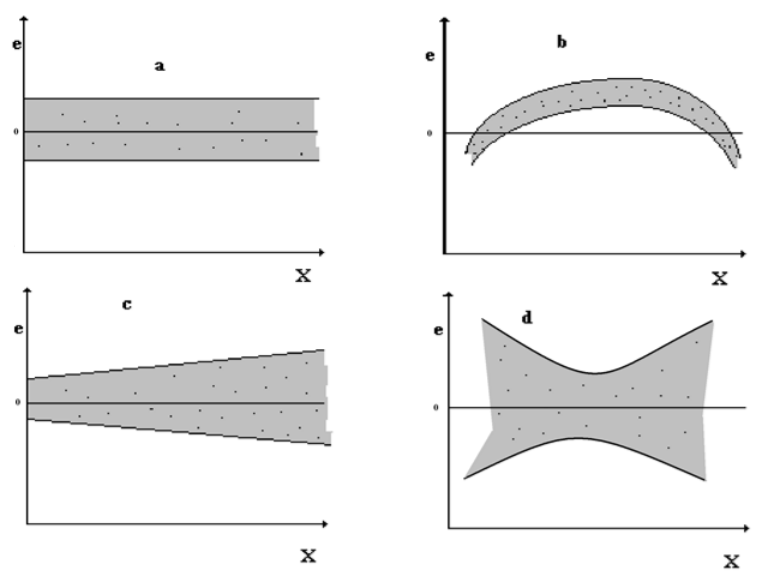
\includegraphics[width=0.5\textwidth]{figures/heteroszkedaszticitas.png} \label{fig:hetero}
\end{figure}

A prediktor változókhoz rendelt \emph{$BETA$ együtthatók} minősítik a változók fontosságát az összefüggésben: minél nagyobb a $BETA$ egüttható abszolútértéke, annál fontosabb a változó. Az együtthatók meghatározása az alábbi összefüggés szerint törénik:

$BETA_i = b_i \cdot \frac{\text{i-dik változó standard szórása}}{\text{célváltozó standard szórása}}$, ahol $b_i$ a regressziós együttható

A meghatározottsági együttható (R-squared) megmutatja, hogy a lineáris regresszióval a célváltozó mekkora hányadát lehet magyarázni. Értéke 0 és 1 között változik, számítása:

$R^2 = \frac{SSR = \Sigma_{i=1}^n\big(\tilde{Y}_i - \bar{Y}  \big)^2}{SSTO = \Sigma_{i=1}^n\big(Y_i - \bar{Y}  \big)^2}$

Az \emph{adjusztált meghatározottsági együttható} segítségével kiküszöbölhetjük azt a problémát, hogy újabb változók bevonásával $R^2$ automatikus nő és túl optimista képet mutat a modell illeszkedéséről. A adjusztált változatban büntetjük a túl sok változó bevonását a modellbe.